% !TEX root ../thesis
\chapter{Evaluation\label{ch:Evaluation}}

\abstract{In this chapter we evaluate the results obtained from dissecting Dridex's \gls{p2p} protocol. First the concept and implementation of the \emph{Dridex L2 Scanner} is briefly highlighted. We then motivate the choice of our data sets and present the results obtained by scanning and monitoring them. Finally, the chapter closes with some security considerations of the \gls{p2p} protocol.}

To verify the knowledge obtained from reverse engineering Dridex's \gls{p2p} protocols the \emph{Dridex L2 Scanner} was written.
As the request for \gls{pl} updates could not be completeley documented, real crawling monitoring was not possible.
However, the scanner is able to identify active L2 nodes with high confidence by sending crafted \gls{p2p} protocol messages and parsing the responses.
In addition a small monitoring component was built to track the online status of discovered \glspl{sp}.

\section{Dridex L2 Scanner\label{sec:Evaluation::Dridex_L2_scanner}}
The \emph{Dridex L2 Scanner} was developed to be able to efficiently detect layer 2 nodes in large \gls{ip} address ranges.
To achieve this, we selected the \emph{CheckMe} process (cf:~\autoref{fig:Communication::Bot_stage::Checkme}) from the \gls{p2p} protocol as basis for the scan since the messages are relatively simple, yet provide strong \glspl{ioc}.
The overall process consists of three phases which are depicted in~\autoref{fig:Dridex_L2_scanner::Phases}.
First, in the \emph{pre-selection} phase, a candidate list is built based on open ports in the scanned \gls{ip}-address range.
In the \emph{probing phase} the scanner probes each selected host with a crafted `\lstinline|checkme|' message (cf:~\autoref{bf:P2P::Request::Checkme}) to check for active L2 nodes.
Ultimately, the list of \glspl{ip} which responded with a correct response on the socket are compared with the list of \glspl{ip} which tried to connect to the scan machine on the announced \gls{p2p} port.
Any matches between these two sets indicate an infection at the specific host. \\

\begin{figure}[htb]
    \centering
    \makebox[\linewidth][c]{
        \begin{tikzpicture}[
            node distance = 0mm and 18mm,
            arrowbox/.style = {arrow box,
                arrow box arrows={east:1cm},
                arrow box shaft width=2.5cm,
                arrow box head extend=0mm,
                line width=0,
                text=white,
                font=\sffamily\bfseries,
                inner sep=5mm,
                minimum height=2.5cm,
                minimum width=8em,
                align=center,
                text width=10em,
            }
        ]
            \flowarrowfirst{S3}{\hspace{1.5em}Verification\\\hspace{1.5em}\small{(correlate \glspl{ip})}}{BrickRed}{white}
            \flowarrow{S2}{\hspace{1.5em}Probing\\\hspace{1.5em}\small{(send `\texttt{checkme}')}}{BurntOrange}{white}{S3}
            \flowarrow{S1}{\hspace{1.5em}Pre-selection\\\hspace{1.5em}\small{(based on ports)}}{ForestGreen}{white}{S2}
        \end{tikzpicture}
    }
    \caption{Dridex L2 scanner phases\label{fig:Dridex_L2_scanner::Phases}}
\end{figure}

\begin{description}
    \item[Pre-selection]
    As highlighted in~\autoref{lst:BindPortForP2P} Dridex uses a set of 13 preferred ports for the \gls{p2p} protocol with a fallback mechanism choosing the first free one between \texttt{1000} and \texttt{65000}.
    We use this information to limit our scan to the hosts that have at least one of the preferred ports open as it is highly unlikely that the fallback routine is used on a regular machine that is not a \gls{sandbox}.
    The goal of this phase is to obtain a list of \glspl{ip} listening on at least one of the 13 preferred ports which are later probed.
    For this phase Zmap\fnote{\url{https://zmap.io}} was used as it provides unparalleled scanning speed for large \gls{ip}-address ranges.
    Unfortunately---due to the architecture of the program---only one port can be scanned at once, which resulted in 13 separate runs.
    \item[Probing]
    In this phase the scanner works through the generated \gls{ip} lists from phase 1 in order of port preference and sends a prepared `\texttt{checkme}' request containing a pre-selected port number.
    A Dridex L2 node will obtain the port number from the message, try to initiate a connection and report back the failure on on the same socket the original request was sent.
    The scanner verifies that the response received on the socket is a valid Dridex \gls{p2p} message and records the \gls{ip} addresses of the hosts.
    Any other responses---such as \gls{http} 404/``Not Found'' or \gls{tls} handshake failures---are discarded and ignored.
    The scanning component was implemented in Python as it provides a decent tradeoff between raw performance and the ability to quickly iterate.
    Its \lstinline|socket| functions are almost exclusively direct wrappers around their native C counterparts guaranteeing a high throughput without manual memory management.
    The verification task of the received Dridex responses was separated into a standalone, executable script to make it available for offline analysis.
    \item[Verification]
    While the scan was running a \emph{tcpdump} process captured attempted connections on the advertised \gls{p2p} port for later correlation.
    Although a valid Dridex \gls{p2p} response on the socket is a very strong \gls{ioc}, we compared the \gls{ip} addresses of these hosts with the list of all hosts that initiated a connection on the specified port.
    The combination of these results indicates that either a real Dridex L2 node is running on that host or a sophisticated \gls{sn} by other security researchers (cf:~\autoref{sec:Related_work::Botnets}).
\end{description}

While the Dridex L2 Scanner was built to detect L2 nodes/\glspl{sp} on the public internet, it can also be used inside private networks to identify regular \glspl{bot}.
This is possible because the \gls{mw} always binds and listens on a port even if not instructed by the \gls{c2} as the port is required for the \emph{CheckMe} process to decide if the \gls{bot} could be a \gls{sp}.
This enables the scanner to find the infected machines given that direct routing is possible and traffic is not filtered by a firewall on the network or host.


\section{Data sets\label{sec:Evaluation::Data_sets}}
We verified the scanner on two data sets using knowledge from the first scan to optimize the second run on a larger \gls{ip}-address range.
Key characteristics of both scans are summarized in \autoref{tab:DataSets}.
The first scan was performed on the large subnets\fnote{All subnets containing more than 4096 addresses (``/20'')} allocated to the Great Britain by \acrshort{ripe}.
These networks were chosen specifically because the country was historically the most damaged region by Dridex~\cite{blueliv2015chasing}.
Of course, this does not necessarily mean that many layer 2 nodes are running in these \gls{ip} address ranges but from an administrative standpoint, it makes sense to deploy at least some \glspl{sp} there to guarantee low latencies for data exfiltration.
This scan included 106,033,152 \gls{ip} addresses which attribute for about 2.5\% of the entire \gls{ip4} address space.
1,676,202 of the scanned \gls{ip} addresses were actually probed with the prepared `\lstinline|checkme|' message, because they listened on one or more of the 13 preferred ports.

\begin{table}
    \centering
    \begin{tabular}{rrr}
        \toprule
        &
        \#1: GB subnets > \texttt{/20} &
        \#2: \gls{ripe} \\
        \midrule
        Total \gls{ip}s &
        106,033,152 (02.47\%)\(^\dag\) &
        814,461,240 (18.96\%)\(^\dag\)\\

        Probed unique \gls{ip}s &
        1,676,202 (00.04\%)\(^\dag\) &
        11,040,833 (00.26\%)\(^\dag\)\\

        Scanned ports &
        all 13 &
        top 4\\

        Bytes send &
        \({\sim}\)3600 MB\(^\ddag\) &
        \({\sim}\)8600 MB\\

        Scan time &
        35:00 hours &
        20:35 hours\\
        \bottomrule
        \multicolumn{3}{l}{\(^\dag\) percentage of the \gls{ip4}-address space} \\
        \multicolumn{3}{l}{\(^\ddag\) estimated value} \\
    \end{tabular}
    \caption{Verification data sets for Dridex L2 Scanner\label{tab:DataSets}}
\end{table}

For the second scan we extended the \gls{ip}-address range to cover all addresses assigned by \gls{ripe} totaling in 814,461,240 \gls{ip}s.
The results obtained from this first data set prompted us to limit this scan to the first four preferred ports (cf:~\autoref{lst:BindPortForP2P}).
Given that Dridex is most prevalent in Europe and with about 19\% of the \gls{ip4} address space scanned, this data set may hint at Dridex's population count.
This run finished significantly faster as the scanner was optimized to open 1024 concurrent connections instead of the previous 256.

\begin{quote}
\textbf{Remark:} The \gls{ip}-address ranges for both data sets were obtained from an official list by \gls{ripe} retrieved from \url{ftp://ftp.ripe.net/pub/stats/ripencc/delegated-ripencc-extended-latest} on the 02.11.2017.
Country allocation was determined solely by the identifier in the second column.
\end{quote}


\section{Results\label{sec:Evaluation::Results}}
After scanning the first data set we received three distinct responses that the scanner categorized as valid Dridex responses.

\begin{description}
    \item[Dridex]
    This category of messages heavily suggests either a Dridex L2 node or a sensor node running on the probed host as the response matched the expected behavior exactly.
    The message returned contained the expected status code ``0404'' which indicates a failed \emph{CheckMe} process.
    As the scanner does not listen on the port specified in the request the node cannot connect to it and returns the error appropriately.
    All of these hosts could also be found when matching the \gls{ip} addresses of these host with the attempted connections on the advertised port.
    Each host tried to establish a connection exactly three times directly after receiving the `\lstinline|checkme|' request further hinting at protocol conform behavior.
    \item[Empty]
    In the first run the scanner marked some \glspl{ip} with an empty response inside the \gls{p2p} envelope (cf:~\autoref{bf:P2P::Envelope}), which was unexpected according to the analyzed Dridex sample.
    At first glance this could point at either poorly implemented \glspl{sn} or perhaps Dridex L2 nodes running a newer version with a changed response format for the `\lstinline|checkme|' request.
    Unfortunately, the scanner hat a bug in parsing responses during the scan of the first data set.
    Responses with a length of exactly 168 bytes were reported as valid but not to have any payload.
    Most probably, all responses in this category come from applications other than Dridex and were wrongly classified because of this bug.
    This is supported by the fact, that we did not observe any more messages of this category during the scan of the second data set with a fixed version of the scanner.
    \item[Echo]
    Several hosts implemented a concept commonly referred to as \emph{Echo Server}.
    Each incoming message is directly sent back to the sender, effectively mirroring the request.
    Because the scanner only detects and unwraps the \gls{p2p} message envelope, the crafted `\lstinline|checkme|' message was classified as valid.
    Although not particularly interesting in itself the hosts did technically send valid Dridex messages which could be monitored by netflow analysis in transit.
\end{description}

\begin{figure}
    \centering
    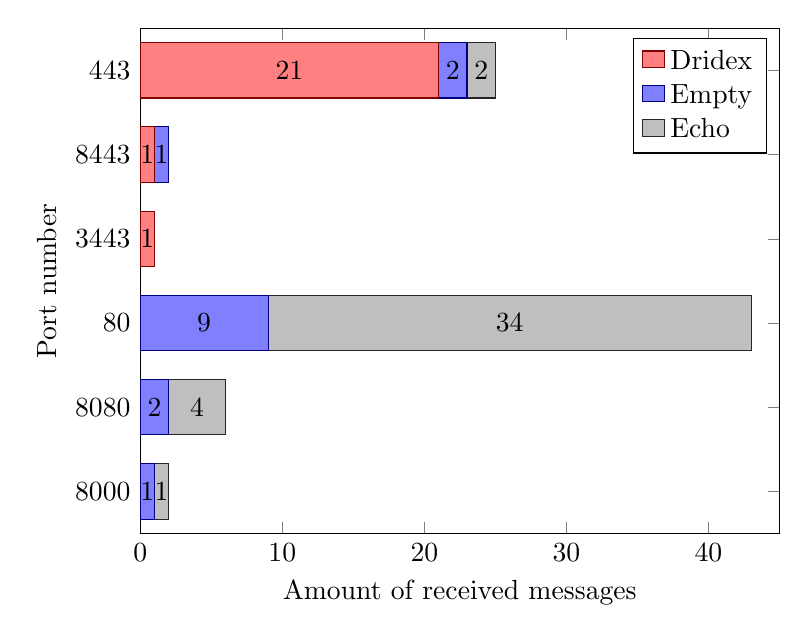
\begin{tikzpicture}
        \begin{axis}[
            xbar stacked,
            ytick=data,
            nodes near coords,
            symbolic y coords={8000,8080,80,3443,8443,443},
            xlabel={Amount of received messages},
            ylabel={Port number},
            enlarge x limits=0,
            xmax=45,
            legend cell align=left,
            height=8cm,
            width=.8\linewidth,
            bar width=20pt]
            \addplot[draw=red!50!black, fill=red!50] coordinates
                {(21,443) (1,8443) (1,3443) (0,80) (0,8080) (0,8000)};
            \addplot[draw=blue!50!black, fill=blue!50] coordinates
                {(2,443) (1,8443) (0,3443) (9,80) (2,8080) (1,8000)};
            \addplot[draw=gray!30!black, fill=gray!50] coordinates
                {(2,443) (0,8443) (0,3443) (34,80) (4,8080) (1,8000)};
            \legend{Dridex, Empty, Echo};
        \end{axis}
    \end{tikzpicture}
    \caption{Dridex L2 Scanner results for data set \#1\label{fig:ScanResults::GB}}
\end{figure}

The results of scanning the first data set are shown in \autoref{fig:ScanResults::GB}.
The majority of the potential Dridex L2 nodes are handling the \gls{p2p} protocol on the port 443 with few exceptions using 8443 and 3443.
This is consistent with the local tests on the analyzed main bot module sample, which would always pick the first free port from the hard-coded list of preferred ports (cf:~\autoref{lst:BindPortForP2P}).
Based on these results all future scans were reduced to only probe the first four ports in the list (443, 8443, 3443, 4443) as it seems highly unlikely that the \gls{mw} would choose a port beyond that.
This is especially true as the ports 3443 and 4443 are assigned to rarely used programs according to \gls{iana}'s database.
It might make sense to consistently scan all preferred ports to detect peers purposefully listening on exotic ports which might be \glspl{sn} or maybe even \glspl{hp} operated by the Dridex \glspl{bm}.
However, even for these use-cases, it seems more efficient to just use a standard port to attract more traffic.

With the results obtained from the first data set the scanner was optimized to directly identify echo servers and discard the wrongly classified empty messages.
The scan of the second data set, the entire address space manageged by \gls{ripe}, revealed more L2 nodes.
After the scan the total L2 node count was 42, only 19 more than the initial 23 found in Great Britain.
This value is especially confusing as some nodes originally found in the first scan were not present anymore in the second scan.
To measure the distribution across the different countries, a \lstinline|whois| query was issued for each \gls{ip} address and filtered by the ``[Cc]ountry'' field.
The absolute results can be found in \autoref{tab:ScanResults::RIPE::Country}, while \autoref{fig:ScanResults:RIPE::Country} shows the percentages.
Interestingly the scan found 10 additional L2 nodes in Great Britain for a total of 33 (or 78.57\% of all infections).
Although we expected a higher percentage due to Dridex's targeting of this area, this value seems comparatively high.
The results of other countries are roughly as expected from the percentage of \gls{ip} addresses with only Ireland beeing slightly overrepresented.

\begin{figure}
    \begin{floatrow}
        \capbtabbox{%
        \begin{tabular}{lrr}
            \toprule
            Country &
            \# \glspl{ip} &
            \# L2 nodes\\
            \midrule
            GB &
            122,734,616 &
            33\\

            FR &
            80,898,864 &
            2\\

            IT &
            53,982,016 &
            1\\

            SE &
            30,079,336 &
            2\\

            NO &
            15,858,064 &
            1\\

            IE &
            6,493,776 &
            2\\

            BG &
            4,440,064 &
            1\\

            \textsc{Rest} &
            499,974,504 &
            0 \\
            \midrule
            \textsc{Total} &
            814,461,240 &
            42\\
            \bottomrule
        \end{tabular}\vspace{.75em}}{\caption{\gls{ripe}: \gls{ip} and L2 node counts per country\label{tab:ScanResults::RIPE::Country}}}
        \ffigbox{%
        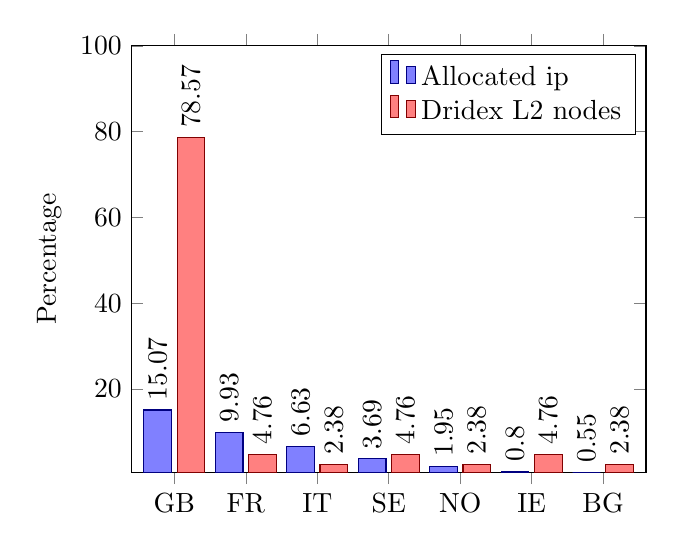
\begin{tikzpicture}
            \begin{axis}[
                ybar,
                xtick=data,
                nodes near coords,
                every node near coord/.append style={rotate=90, anchor=west},
                symbolic x coords={GB,FR,IT,SE,NO,IE,BG},
                ylabel={Percentage},
                enlarge y limits={upper,value=0.275},
                legend cell align=left,
                height=7cm,
                bar width=10pt]
                \addplot [draw=blue!50!black, fill=blue!50] coordinates {
                    (GB,15.069423807080125753)
                    (FR,9.932807115535663797)
                    (IT,6.627941680809758362)
                    (SE,3.693157454613800897)
                    (NO,1.947061839308645308)
                    (IE,0.797309396822861699)
                    (BG,0.545153505401926800)
                };
                \addplot [draw=red!50!black, fill=red!50] coordinates {
                    (GB,78.571428571428571429)
                    (FR,4.761904761904761905)
                    (IT,2.380952380952380952)
                    (SE,4.761904761904761905)
                    (NO,2.380952380952380952)
                    (IE,4.761904761904761905)
                    (BG,2.380952380952380952)
                };
                \legend{Allocated \glspl{ip}, Dridex L2 nodes};
            \end{axis}
        \end{tikzpicture}}{\caption{\gls{ripe}: \gls{ip} and L2 node percentages per country\label{fig:ScanResults:RIPE::Country}}}
    \end{floatrow}
\end{figure}

There are two possible explanations for the unexpected distribution of L2 nodes in Great Britain and the low total number of \glspl{sp} in the \gls{ripe} subnets.
On the one hand, the total number of \gls{ip} addresses per country is calculated by summing up the subnet numbers given in the original file from \gls{ripe} while the country allocation of the infected hosts was determined via \lstinline|whois|.
This could lead to differences, e.g., in cases where an \gls{ip} address is allocated to another country which then resells it to a company or private customer in Great Britain, resulting in a changed \lstinline|whois| entry.
On the other hand, we later discovered that the maximum socket count in the probing phase for the \gls{ripe} data set was set too high which might have resulted in packet drops, possibly missing positive response messages.
Due to time constraints the scan could not be repeated in time but the obtained results should provide a general indication of Dridex's presence in Europe.

\begin{figure}
    \centering
    \begin{tikzpicture}
        \begin{axis}[
            % Type
            %only marks,
            % Setup
            table/col sep=comma,
            date coordinates in=x,
            date ZERO=2017-11-12,
            % Labels
            xlabel={Time of day},
            xticklabel={\hour:\minute},
            xticklabel style={rotate=30, anchor=near xticklabel},
            enlarge x limits=.025,
            ylabel={\# of online L2 nodes},
            xtick distance={0.125},
            ytick distance=2,
            legend pos=north west,
            legend cell align=left,
            % Misc
            width=15cm]
            \addplot+[mark=x, draw=gray, line width=1.25pt] table[x=ts,y=avg] {data/crawler.csv};
            \addplot+[mark=x, draw=blue!50] table[x=ts,y=min] {data/crawler.csv};
            \addplot+[mark=x, draw=red!70] table[x=ts,y=max] {data/crawler.csv};
            \addplot+[mark=none, draw=gray!50, line width=1pt, dashed] table[x=ts,y=total_avg] {data/crawler.csv};
            \legend{Average, Min, Max, Total average}
        \end{axis}
    \end{tikzpicture}
    \caption{Active L2 nodes during the day between 12.--15.11.2017\label{fig:CrawlingResults}}
\end{figure}

To gain more insights about the uptime of the detected L2 nodes, the probing component was adapted to use a newly crafted `\lstinline|ping|' request message (cf:~\autoref{bf:P2P::Request::Ping}).
This request type was chosen over the previously used `\lstinline|checkme|' as it does not prompt the L2 node to initiate a connection improving the response time.
Additionally, the `\lstinline|pong|' response contains the node's BotId delivering even more data to analyze.
\autoref{fig:CrawlingResults} shows the results obtained from checking the online status of the known bots between 12.11.2017--15.11.2017.
The x-axis shows the time of day from 00:00 to 24:00; the plot illustrates the average, minimum and maximum number of active L2 nodes measured for any given 15 minutes among all four days.
From the 42 unique \glspl{ip} found only a total of 24 were online at peak times during the monitoring process.
This can be attributed to \gls{node_churn} or non-static \gls{ip} addresses (very common in non-professional connection setups).
As the request for \gls{pl} updates could not be reverse engineered this remains a problem in the current monitoring approach.

Although the monitoring window was very short, a trend is visible showing more active \glspl{sp} during typical work hours and slightly past that.
Especially visible is the sharp rise at 09:00 passing the total average of 16 active \glspl{sp} and the steady decline starting at around 16:00.
This seems to indicate that at least some of the crawled L2 nodes are running on office computers which get shut down later in the day.
However, longer crawling timespans and a larger set of known \glspl{ip} are definitely required to verify this claim.

Another interesting fact was revealed when BotIds were crawled for all known infected hosts.
A set of 5 closely related \gls{ip} addresses (in the same ``/29'' subnet) all returned the exact same BotId: \lstinline|OFFICE_4ecea422c76a2a58da6e42c7c47f283c|.
The clash heavily implies either a cloned \gls{vm} instance, a machine that is available from multiple \gls{ip} addresses or a simple \gls{sn}/\gls{hp} implementation with a hard-coded setting for this property because this value is computed from unique values of the Windows registry 
As a \lstinline|whois| query did not immediately reveal a particular research or commercial entity behind the hosts, this theory could not be confidently verified.

    %IE 6493776
    %PL 20868168
    %BE 28447104
    %SE 30079336
    %ES 30521664
    %RU 45087744
    %NL 47058400
    %IT 53982016
    %FR 80898864
    %DE 120098432
    %GB 122734616

    % 814461240

    % 33 GB
    %  2 FR
    %  2 IE
    %  2 SE
    %  1 IT
    %  1 BG
    %  1 no

\section{Security considerations\label{sec:Evaluation::Security_considerations}}
When analyzing the communication protocols and especially the \gls{p2p} protocol we found two minor weaknesses that might be useful in monitoring and takedown attempts.
While none of them is trivially exploitable they still present significant opportunities for possible takedown attempts.

\begin{description}
    \item[Missing buffer length validation]
    In several places the functions responsible for protocol handling use length values directly read from a message without verifying that the message buffer actually contains the requested amount of data.
    While the envelope handling is quite robust---discarding all invalid messages reliably---the actual message handling often relies valid messages.
    One example is the encrypted BotId that is mandatory in every \gls{p2p} request (cf:~\autoref{bf:P2P::Request}).
    If the encoded string is omitted the following message content is directly interpreted as a length argument leading to an \emph{access violation} terminating the execution.
    This is not as critical as one might imagine as each incoming connection gets handled in a newly spawned thread, but it nonetheless demonstrates that the binary contains possibly exploitable vulnerabilities.
    \item[Protocol inconsistency]
    As mentioned above the `\lstinline|ping|' message was used to continuously crawl the known L2 nodes.
    This message is only used to check whether a new \gls{bot} can be promoted to a \gls{sp}.
    Since the L2 nodes are already \glspl{sp} they should not even be required to handle this request type unless it is also used for some kind of \gls{c2} heartbeat.
    Unfortunately the analysis did not cover the \gls{c2} protocol but it seems unlikely that a layer 3 node (or even the \gls{c2}) would use a request from the \gls{p2p} protocol for such a purpose.
    Until this inconsistency is addressed, the `\lstinline|ping|' request remains a good way to cheaply detect the online status of L2 nodes and retrieve their BotId which is also included in the `\lstinline|pong|' response.
\end{description}


\section{Summary\label{sec:Evaluation::Summary}}
The Dridex L2 scanner is able to reveal active L2 nodes in large \gls{ip}-address spaces in reasonable time.
With the detection of 42 \glspl{sp} throughout the European \gls{ip}-address space we have strong indications that the protocol descriptions presented earlier are accurate for the sample that we analyzed.

As only one sample of the main bot module was dissected it cannot be verified that this protocol is generally used by all Dridex subnets.
However, the presence of active L2 nodes in multiple countries---8 month after the sample was discovered in the wild---suggest that multiple subnets still use the exact protocol today.
Additionally, the set of L2 nodes was monitored for a short amount of time, revealing a pattern in their uptime which indicates that some of them are running in office environments.
This assumption could be further verified by extended monitoring across a larger timeframe.